\documentclass[legalpaper,12pt]{article}
\usepackage[utf8]{inputenc}
\usepackage[T1]{fontenc}
\usepackage{caption}
\usepackage[document]{ragged2e}
\usepackage[english]{babel}
\usepackage{vmargin}
\usepackage{textcomp}
\usepackage{graphicx}
\usepackage{lscape}
\usepackage{hyperref}
\usepackage{multirow}
\setmargins{2.5cm}% margen izquierdo
{1.5cm}% margen superior
{16.5cm}% anchura del texto
{23.42cm}% altura del texto
{10pt}% altura de los encabezados
{1cm}% espacio entre el texto y los encabezados
{0pt}% altura del pie de página
{2cm}% espacio entre el texto y el pie de página

\graphicspath{{images/}}
\parskip=5pt
\begin{document}
%%%%%%%%%%%%%%%%%%
%%% Inicio %%%
%%%%%%%%%%%%%%%%%%
\begin{titlepage}
    \begin{center}
        
\includegraphics[width=1\textwidth]{logo}\\[3cm]
        {\large Computer School}\\[1cm]
        {\large Prof: Dr. Francisco J. Torres Rojas}\\[2cm]
        {\huge Project 0}\\[1cm]
        {\huge Old-fashioned multiplication }\\[1cm]
        \rule{\linewidth}{0.5mm} \\[0.4cm]
        { \huge \bfseries  Technical Report \\[0.4cm] }
        \rule{\linewidth}{0.5mm} \\[1.5cm]
        \center{José Ceciliano Granados 2016087245
              \\Luis Alejandro Garita 2016094679}  
        \vfill
        {\large Version 1.0 \\ \today}
    \end{center}
\end{titlepage}
\newpage

%%%%%%%%%%%%%%%%%%%%%%%%%%%%%%%%%%%%%%%%%%%%
%%% Index
%%%%%%%%%%%%%%%%%%%%%%%%%%%%%%%%%%%%%%%%%%%%
\renewcommand*\contentsname{Index}
\tableofcontents
\newpage

%%%%%%%%%%%%%%%%%%%%%%%%%%%%%%%%%%%%%%%%%%%%
%%% Introduction
%%%%%%%%%%%%%%%%%%%%%%%%%%%%%%%%%%%%%%%%%%%%
\section{Introduction}
\justifying
The search of this report is to make an analysis on the data gathered in tests of how long does it take for a computer to do different multiplication versions by a certain number of times, always with the same random numbers. There will be three different multiplications versions used for this report:
\begin{enumerate}
    \item Empty version, the function only return zero.
    \item Standard version, the function uses the language usual multiplication method (i.e. A * B).
    \item Ancient version, this algorithm uses an old algorithm explained in the project specification.
\end{enumerate}
\justifying
To make a more interesting analysis, the three methods showed before will be made in two different languages. First in a high level language as C, and then in a low level language as assembler, in this case NASM. 

\newpage


%%%%%%%%%%%%%%%%%%%%%%%%%%%%%%%%%%%%%%%%%%%%
%%% Structure
%%%%%%%%%%%%%%%%%%%%%%%%%%%%%%%%%%%%%%%%%%%%

\section{Program Structure}

\subsection{Basics}
\justifying
As explained before, the idea is to repeat each method of multiplication a number N times and get the time it took for each method to finish the process. Before starting is necessary to know and understand the global variables that will be used in the program. Now the first step is to get the random generated numbers that will be used over and over for every multiplication method, and save them in a variable. The second step is to print for the user the tables that will be used for the program first in the form A*B and later in the form B*A. Next step is do each multiplication step N times and show the results and times in screen for A*B and vice versa. And last but not least wait for the user to press a key to see the next method. For an example run of the program, please check the annexes 1 through 7\\ [0.5cm]

\subsection{Variables}
The program uses the following global variables:
\begin{itemize}
    \item clock\_t tInicio: Used to take the time when the function starts.
    \item clock\_t tFin: Used to take the time when the function finishes.
    \item clock\_t tDecorrido: Will have the time between tInicio and tFin.
    \item int num\_aleatorio[7]: Is a list with the 8 random generated numbers.
    \item int mat[4][4]: Is a matrix of 4 by 4 that saves the result of the operation.
    \item int n=10000000: Is the n with the amount of times the user wants to repeat each operation.
\end{itemize}

\begin{center}{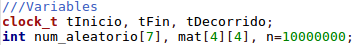
\includegraphics[width=0.75\textwidth]{Variables.png}\\[1cm]}\end{center}


\subsection{Multiplication Functions}
The functions for multiplication made in C where the following in the order empty, standard and ancient:
    
\begin{center}{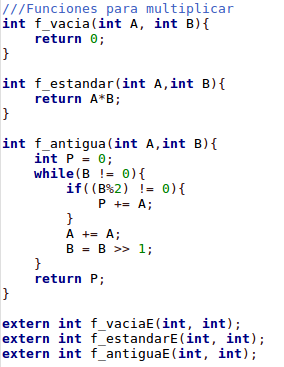
\includegraphics[width=0.5\textwidth]{funcionesC.png}\\[1cm]}\end{center}

\justifying
Notice that the last three are just defining that those functions will exist, the extern implies those three are actually programmed in assembler as follows:

\begin{center}{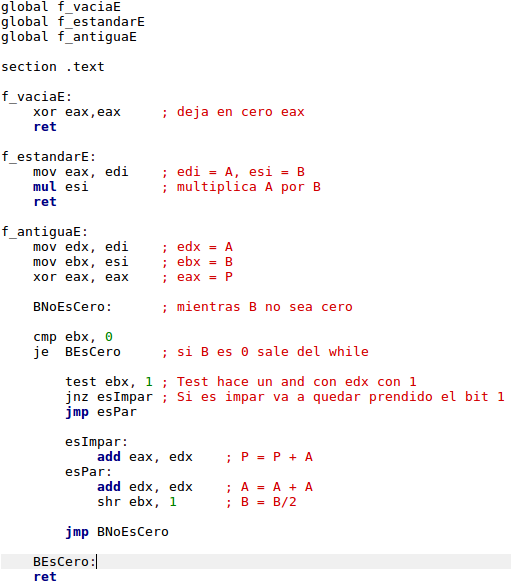
\includegraphics[width=0.5\textwidth]{funcionesNASM.png}\\[1cm]}\end{center}


\subsection{Writing Functions}
\justifying
To make sure all the times and random generated numbers were properly saved in a text file, there are a few functions dedicated only to the matter. This helped a lot in the process of analysing the data. They were the following:

\begin{center}{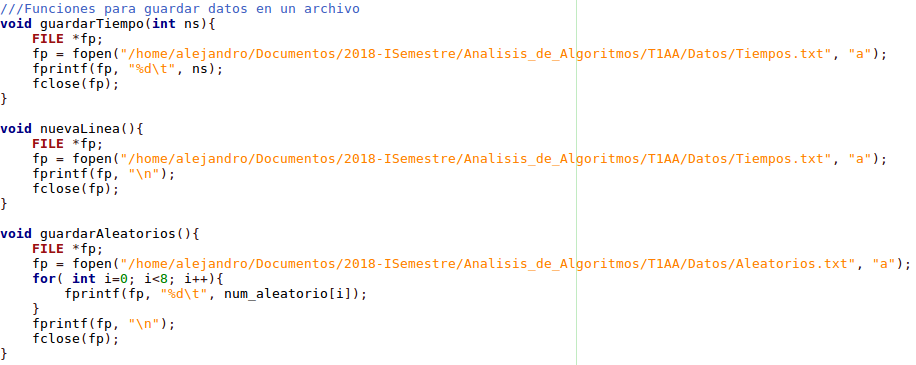
\includegraphics[width=1\textwidth]{escribir.png}\\[1cm]}\end{center}


\subsection{Interface functions}
\justifying
One of the most important parts of the program is to show the data obtained to the user. So that's why there are a lot function which purpose is to show the interface in a nice and clear way. The most important interface functions will be explained.

\begin{itemize}
    \item escribir\_base: It writes the two matrices used, not with the results but with the operands used, in both A*B and B*A.
    \begin{center}{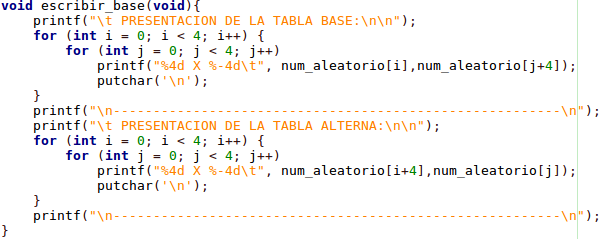
\includegraphics[width=0.75\textwidth]{escribirBase.png}\\[1cm]}\end{center}
    \item escribir: In this case it presents both matrices results, plus the time it took for it to finish.
    \begin{center}{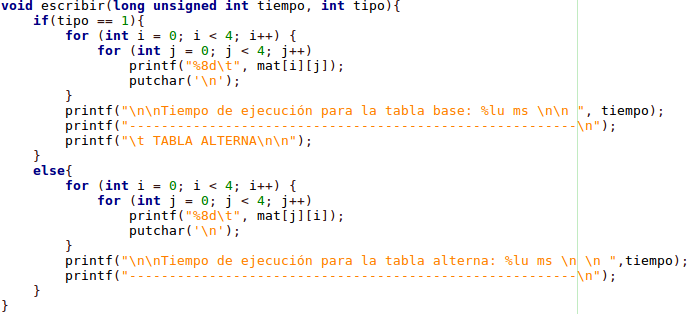
\includegraphics[width=0.75\textwidth]{escribirResp.png}\\[1cm]}\end{center}
    \item escribir\_num\_aleatorio: This one just prints the 8 random numbers used.
    \begin{center}{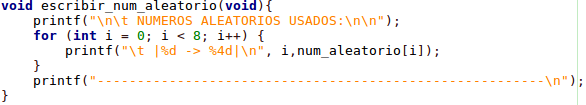
\includegraphics[width=0.75\textwidth]{escribirRand.png}\\[1cm]}\end{center}
    \item siguiente: This one is really important, it waits for the user to press enter so the program can continue.
    \begin{center}{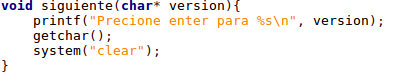
\includegraphics[width=0.75\textwidth]{siguiente.png}\\[1cm]}\end{center}
    \item versionVaciaC: For this functions where NNNN is the versions name and L the language. This are the most important because they are ones that actually call the multiplication functions and store the result in the matrix. Only one will be shown because all of them are very similar.
    \begin{center}{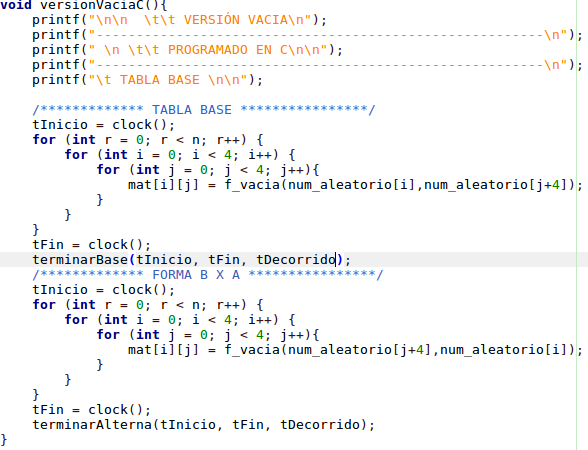
\includegraphics[width=0.75\textwidth]{ejemploVersion.png}\\[1cm]}\end{center}
\end{itemize}


\subsection{Others}
There were other important functions used.
\begin{itemize}
    \item terminar: this functions finished the run of one of the methods and is where the time is calculated.
    \begin{center}{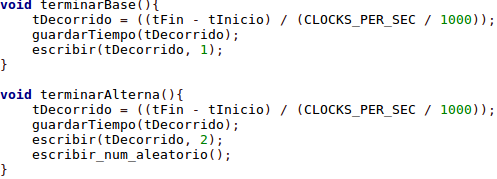
\includegraphics[width=0.75\textwidth]{terminar.png}\\[1cm]}\end{center}
    \item main: This is the principal function, that starts the program and call the rest of the functions
    \center{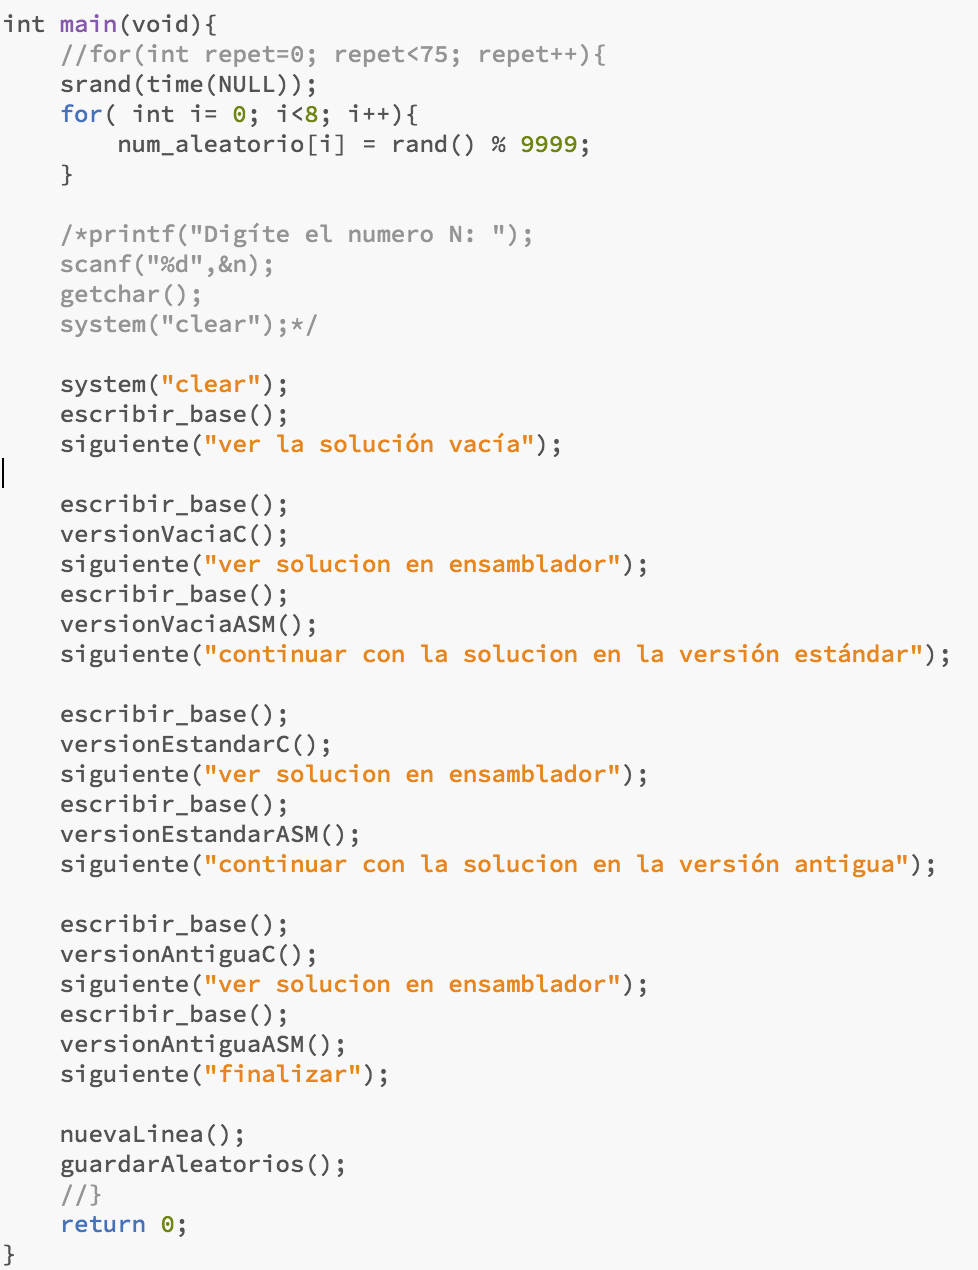
\includegraphics[width=1\textwidth]{main.png}\\[3cm]}
\end{itemize}
\newpage


%%%%%%%%%%%%%%%%%%%%%%%%%%%%%%%%%%%%%%%%%%%%
%%% Results
%%%%%%%%%%%%%%%%%%%%%%%%%%%%%%%%%%%%%%%%%%%%

\section{Data Analysis}
\justifying
Now is presented three table with interesting data obtained for the program after the use of a N number of one million and 100 tests. There's data such as the highest time, the lowest time, the average time, the difference between the highest and lowest, the most repeated time and how many times it repeated. Also there will be a deeper analysis from the data obtained for each version of the program. For the full table, check in annexes for table 8.1, 8.2 and 8.3. 

\subsection{Considerations}
    \justifying
    For this test, the specifications and operating system of the computer in which the tests were carried out are taken into account, which are:
    
    \begin{itemize}
        \item OS:   Ubuntu 16.04.03 
        \item RAM Memory:   12056MB
        \item Processor:    Intel Core i7-6500U CPU @ 2.50GHz 
    \end{itemize}
    
    \subsubsection{The N number choice}
        \justifying
        Before starting all the tests, there was the idea of trying the program with 500 thousand, 1 million or 10 million times to see which one could give significant data without during an eternity. The discarded ones were 500 thousand because the information it gave wasn't significant enough and 10 million because it was too slow, and for the amount of test that were planned, it wasn't good enough. So at the end the test with a N of 1 million, were really fast and give some interesting information that could be work on.
    \subsubsection{The amount of tests}
        \justifying
        To have a significant amount of data there was needed to run the program a lot of times, and after a little deliberation between the members of the project it was defined that 100 tests would give enough information for this analysis.
\newpage

\subsection{Empty Version}
    \begin{table}[h]
        \caption{Empty Version Data}
        \centering
        \begin{tabular}{|l|l|l|l|l|}
        \hline
        \multirow{3}{*}{}       & \multicolumn{4}{c|}{Empty}                        \\ \cline{2-5} 
                                & \multicolumn{2}{c|}{C} & \multicolumn{2}{c|}{ASM} \\ \cline{2-5} 
                                & AXB        & BXA       & AXB         & BXA        \\ \hline
        Higher                  & 98         & 67        & 82          & 52         \\ \hline
        Average                 & 83.50      & 65.37     & 68.54       & 49.11      \\ \hline
        Lower                   & 64         & 62        & 53          & 48         \\ \hline\hline
        Lower-Higher Difference & 34         & 5         & 29          & 4          \\ \hline\hline
        Most repeated           & 89         & 66        & 77          & 49         \\ \hline
        Times repeated          & 16         & 40        & 17          & 67         \\ \hline
        \end{tabular}
        \label{resultados1}
    \end{table}
    \justifying
    It might be expected that this version will be basically immediate, however, it averages a time of 83.5ms for A*B and 65.3ms for the operations written in Language C, this operation is the result of what the program takes to communicate with the operating system and create a space in memory that returns a 0, what we can observe is the response time of the memory and as though it does not perform any significant function it shows at the time that we are limited by access to memory.
    \justifying    
    At the same time we have the comparison with the assembly language which averages 68.5ms for A*B and 49.1 for B*A, which shows the limitation of the time of access to memory, but still shows a better time in a low level language in comparison to the high level counterpart.
    
    \subsubsection{What is the empty version of the algorithms for?}
        \justifying
        It doesn't really serves a purpose, because as it has been shown it always return 0 so it never does anything. But as the testing has shown it does takes time to do, and that's why the empty function is good it show how long does it takes for the computer to access memory and return a value, in this case 0. 
\newpage

\subsection{Standard Version}
    \begin{table}[h]
        \caption{Standard Version Data}
        \centering
        \begin{tabular}{|l|l|l|l|l|}
        \hline
        \multirow{3}{*}{}       & \multicolumn{4}{c|}{Standard}                     \\ \cline{2-5} 
                                & \multicolumn{2}{c|}{C} & \multicolumn{2}{c|}{ASM} \\ \cline{2-5} 
                                & AXB        & BXA       & AXB         & BXA        \\ \hline
        Higher                  & 107        & 75        & 85          & 53         \\ \hline
        Average                 & 90.16      & 71.86     & 73.26       & 52.45      \\ \hline
        Lower                   & 74         & 71        & 56          & 52         \\ \hline\hline
        Lower-Higher Difference & 33         & 4         & 29          & 1          \\ \hline\hline
        Most repeated           & 78         & 72        & 82          & 52         \\ \hline
        Times repeated          & 15         & 73        & 15          & 55         \\ \hline
        \end{tabular}
        \label{resultados2}
    \end{table}
    \justifying
    We observe an average a little bit higher to the one in the empty function (between 5 and 10 ms slower). For the standard multiplication operation in C language, we have an average of 90.1ms in A*B and 71.8ms for B*A which shows the access time to memory plus the calculation of Multiplication processing, using the algorithm imposed by the compiler. \\
    \justifying
    Now if we focus on the assembly counterpart we observe a really good result which shows an average of 73.2ms for A*B and 52.45 for B*A, this can be deduced to the memory access time and that working in the registers themselves is a lot faster in assembler which reduces use other system resources to perform the calculation, making it faster.\\
\newpage

\subsection{Ancient Version}
    \begin{table}[h]
        \caption{Ancient Version Data}
        \centering
        \begin{tabular}{|l|l|l|l|l|}
        \hline
        \multirow{3}{*}{}       & \multicolumn{4}{c|}{Ancient}                      \\ \cline{2-5} 
                                & \multicolumn{2}{c|}{C} & \multicolumn{2}{c|}{ASM} \\ \cline{2-5} 
                                & AXB        & BXA       & AXB         & BXA        \\ \hline
        Higher                  & 691        & 665       & 478         & 482        \\ \hline
        Average                 & 639.27     & 608.59    & 422.88      & 408.68     \\ \hline
        Lower                   & 549        & 528       & 366         & 340        \\ \hline\hline
        Lower-Higher Difference & 142        & 137       & 112         & 142        \\ \hline\hline
        Most repeated           & 622        & 623       & 416         & 428        \\ \hline
        Times repeated          & 3          & 8         & 5           & 5          \\ \hline
        \end{tabular}
        \label{resultados3}
    \end{table}
    \justifying
    This function shown by the J.Nyberg paper shows that the average C language time is 639.2ms for A*B and 608.5ms for B*A, far exceeding the result of the multiplication algorithm of the system, this because these instructions require the interpretation and storage of more variables in memory at the same time that requires the use of processing and access to memory, which undoubtedly makes it an inefficient algorithm for multiplication. \\
    \justifying
    For assembly language we have an average of 422.88ms for A*B and 408.6 in B*A which leads us to think that said language, again by being low level and working directly in the registers, requires a greater amount of resources than the standard multiplication method, but makes it faster than the on programmed in C. \\
    
    \subsubsection{Is the ancient algorithm good? How much?}
        \justifying
        After all the tests done, it's safe to say that the ancient algorithm is not good for computers. Actually it's way worse than the standard version, in the case of C is close to 10 times worse. This doesn't mean that this version is completely bad, is just that in the specific case for computers is not good enough, for example, in some cases it might be faster than the standard version for some humans without a calculator.
\newpage

\subsection{Other Information}
    \subsubsection{Is there gain in assembler versions?}
        \justifying
        Yeah, there is and is actually quite significant This is a list with how much percent faster is the assembler version against the C version:
        \begin{itemize}
            \item Empty Version (A*B): 17.91\% faster
            \item Empty Version (B*A): 24.87\% faster
            \item Standard Version (A*B): 18.74\% faster
            \item Standard Version (B*A): 27.01\% faster
            \item Ancient Version (A*B): 33.85\% faster
            \item Ancient Version (B*A): 32.85\% faster
        \end{itemize}
        \justifying
        This shows perfectly that the assembler version is way faster than his counterpart versions in C
        
    \subsubsection{Does the order of the arguments affect? There are some rule?}
        \justifying
        Unexpectedly enough B*A is a lot faster than A*B in all six versions, either NASM or C.
        \begin{itemize}
            \item Empty Version (C): 21.71\% faster
            \item Empty Version (NASM): 28.35\% faster
            \item Standard Version (C): 20.30\% faster
            \item Standard Version (NASM): 28.41\% faster
            \item Ancient Version (C): 4.80\% faster
            \item Ancient Version (NASM): 3.36\% faster
        \end{itemize}
        Even in the ancient version is still faster, not by a great margin though. But in the cases of the empty and the standard version, the difference is significant. It's even more in the NASM versions of the previously said ones.
    \subsubsection{Interesting Data}
        From all the data there are some interesting occurrences, that will be shown now:
        \begin{itemize}
            \item The Standard, NASM, in both versions is so fast that, is even faster than Empty, C, in both versions.
            \item The most consistent version: This achievement goes to the Standard, C, B*A version. In this version the most repeated time is 72ms and is repeated a whopping 73 times in 100 tests.
            \item The least variable version: The Standard, NASM, B*A version. In this version, in all the 100 tests, there were only two different times 52ms and 53ms, no more nor less.
            \item The most variable version: The Ancient, C, A*B version, which is also the slowest, is the one with most variables. It's also the least consistent version, the most repeated time was 622ms with only 3 times from the 100 tests.
        \end{itemize}
\newpage

%%%%%%%%%%%%%%%%%%%%%%%%%%%%%%%%%%%%%%%%%%%%
%%% Annexes
%%%%%%%%%%%%%%%%%%%%%%%%%%%%%%%%%%%%%%%%%%%%
\section{Annexes}

\begin{figure}[htbp]
  \centering
    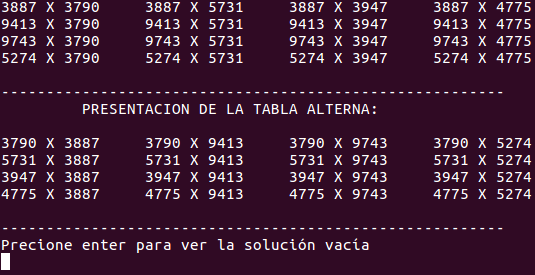
\includegraphics[width=0.75\textwidth]{Inicio.png}
  \caption{Presentation of the numbers generated that will be multiplied}
  \label{fig:Inicio}
\end{figure}


\begin{figure}[htbp]
  \centering
    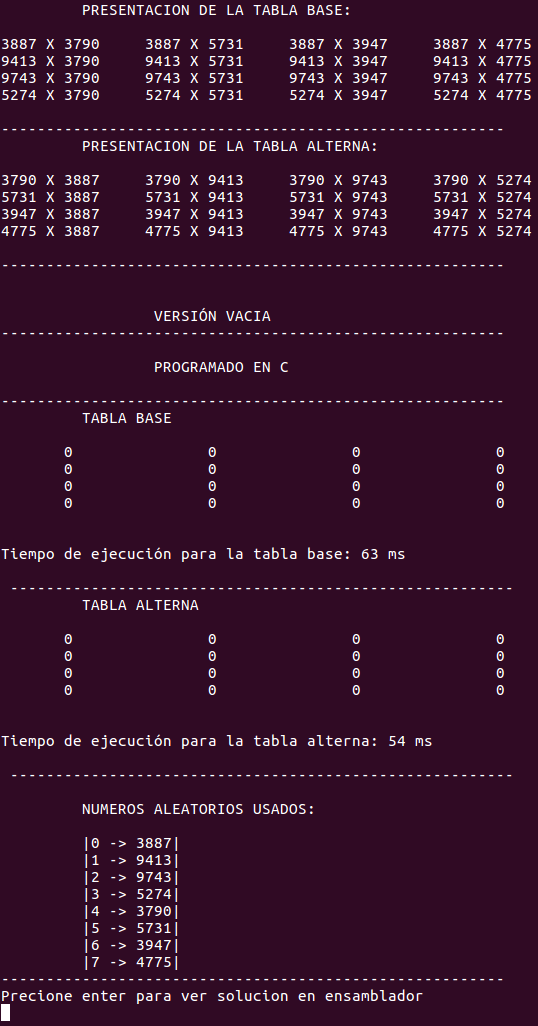
\includegraphics[width=0.75\textwidth]{Vacia_C.png}
  \caption{Empty function programmed in C language}
  \label{fig:vacia_c}
\end{figure}

\begin{figure}[htbp]
  \centering
    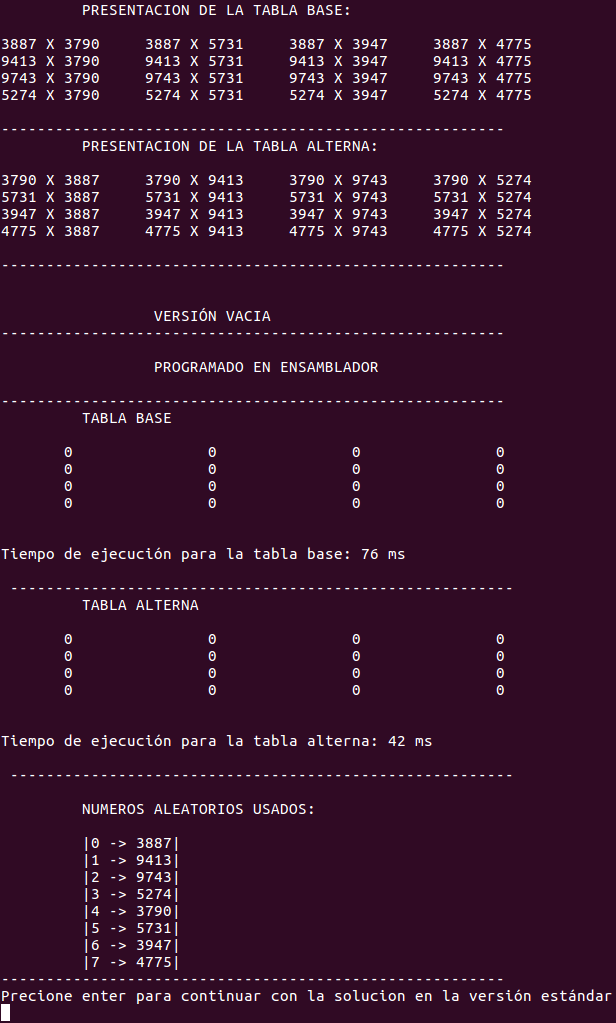
\includegraphics[width=0.75\textwidth]{Vacia_E.png}
  \caption{Empty function programmed in Assembler Language}
  \label{fig:vacia_e}
\end{figure}

\begin{figure}[htbp]
  \centering
    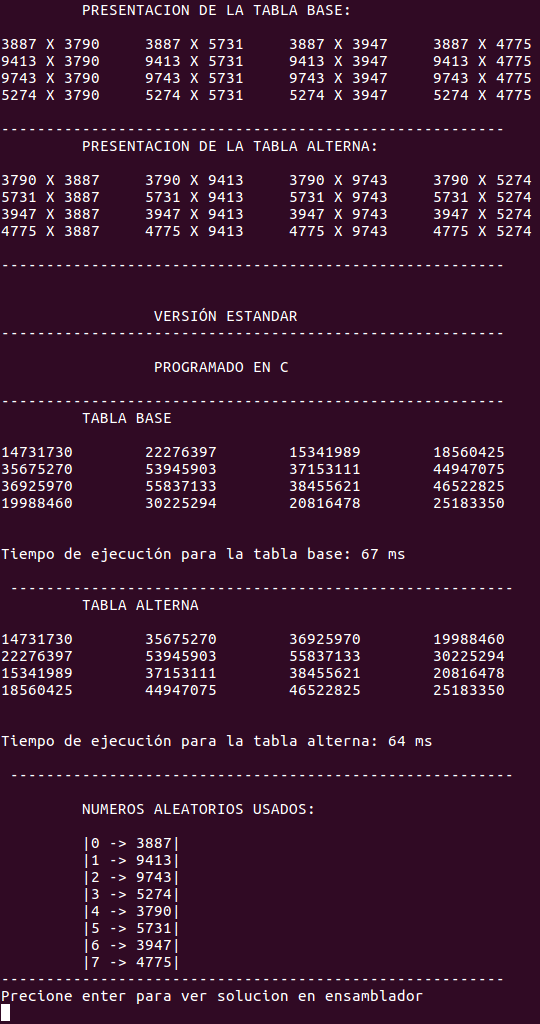
\includegraphics[width=0.75\textwidth]{Normal_C.png}
  \caption{Standard function programmed in Assembler Language}
  \label{fig:normal_c}
\end{figure}

\begin{figure}[htbp]
  \centering
    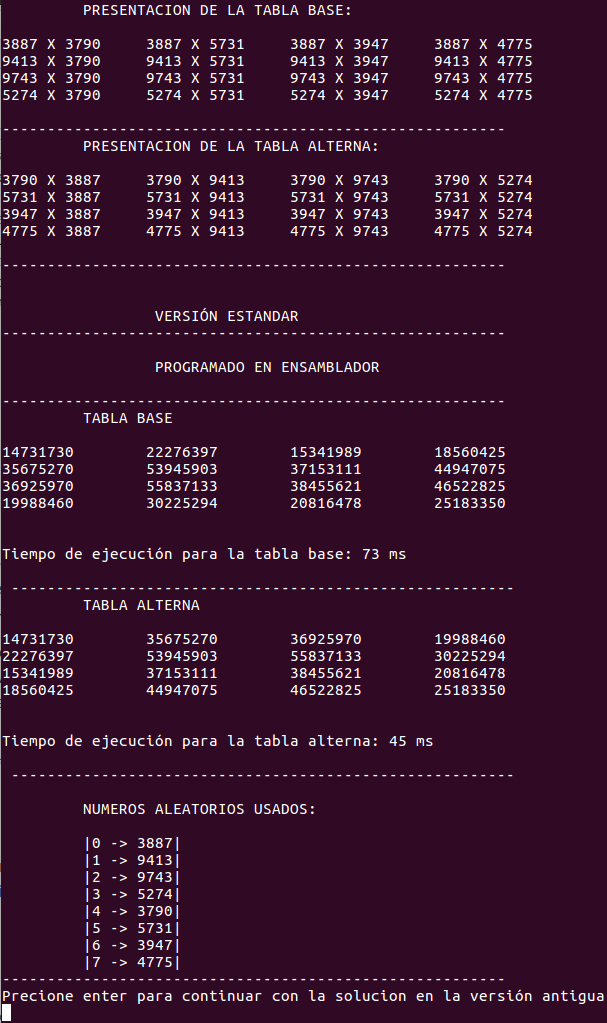
\includegraphics[width=0.75\textwidth]{Normal_E.png}
  \caption{Standard function programmed in C language}
  \label{fig:normal_e}
\end{figure}

\begin{figure}[htbp]
  \centering
    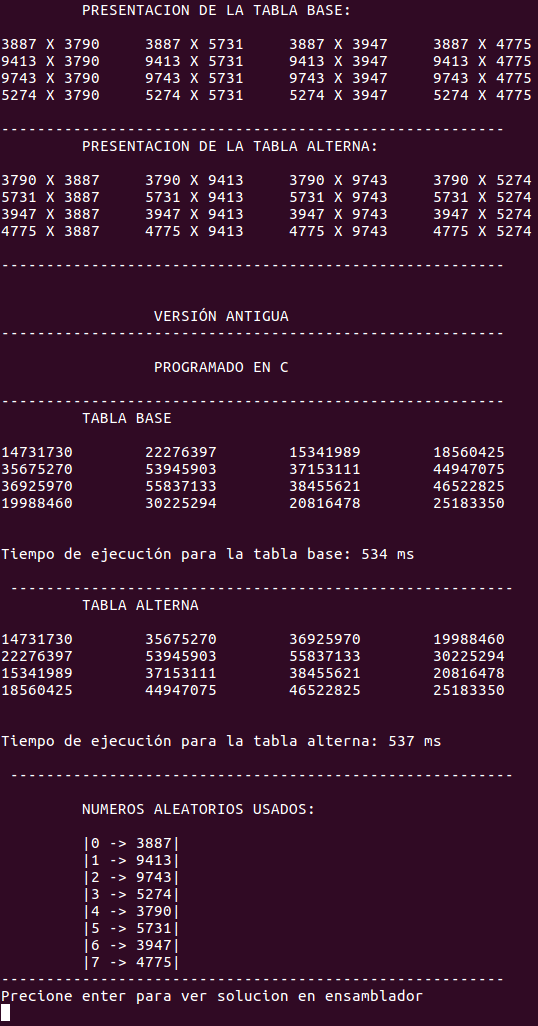
\includegraphics[width=0.75\textwidth]{Antigua_C.png}
  \caption{Ancient function programmed in C Language}
  \label{fig:antigua_c}
\end{figure}

\begin{figure}[htbp]
  \centering
    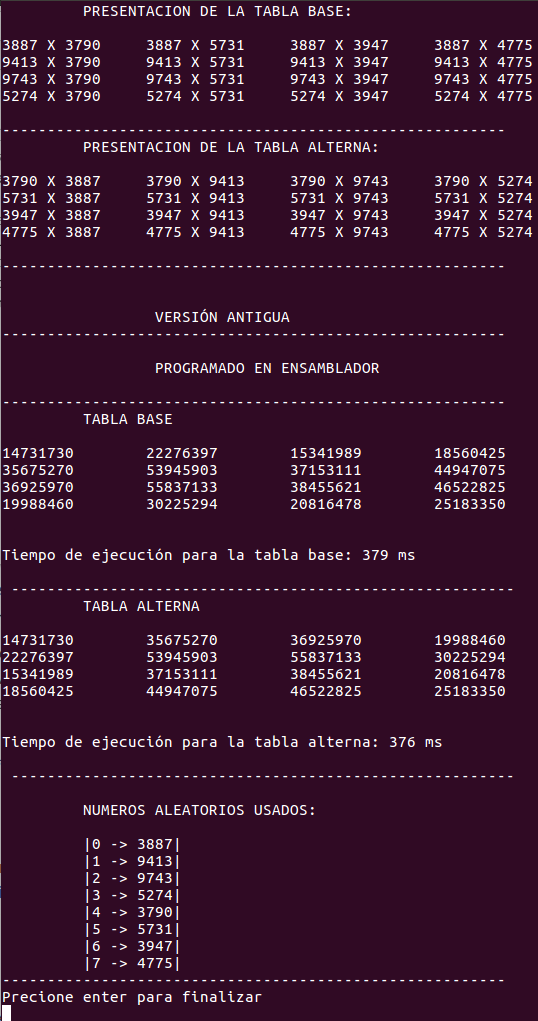
\includegraphics[width=0.75\textwidth]{Antigua_E.png}
  \caption{Ancient function programmed in Assembler Language}
  \label{fig:antigua_e}
\end{figure}

\begin{table}[htbp]
\caption*{Data obtained 8.1}
\begin{tabular}{|l|l|l|l|l|l|l|l|l|l|l|l|l|}
\hline
\multicolumn{1}{|c|}{\multirow{4}{*}{\#}} & \multicolumn{12}{c|}{Time per version}          \\ \cline{2-13} 
\multicolumn{1}{|c|}{}                    & \multicolumn{4}{c|}{Empty}                       & \multicolumn{4}{c|}{Standard}                    & \multicolumn{4}{c|}{Ancient}                        \\ \cline{2-13} 
\multicolumn{1}{|c|}{}                    & \multicolumn{2}{c|}{C} & \multicolumn{2}{c|}{ASM} & \multicolumn{2}{c|}{C} & \multicolumn{2}{c|}{ASM} & \multicolumn{2}{c|}{C} & \multicolumn{2}{c|}{ASM} \\ \cline{2-13} 
\multicolumn{1}{|c|}{}                    & AXB        & BXA       & AXB         & BXA        & AXB        & BXA       & AXB         & BXA        & AXB        & BXA       & AXB         & BXA        \\ \hline
1                                         & 93         & 63        & 63          & 50         & 101        & 72        & 81          & 52         & 666        & 592       & 421         & 421        \\ \hline
2                                         & 70         & 62        & 76          & 50         & 81         & 74        & 83          & 52         & 627        & 624       & 436         & 418        \\ \hline
3                                         & 87         & 63        & 60          & 49         & 99         & 72        & 81          & 53         & 622        & 567       & 402         & 365        \\ \hline
4                                         & 87         & 63        & 80          & 49         & 97         & 72        & 84          & 53         & 663        & 623       & 422         & 428        \\ \hline
5                                         & 90         & 63        & 76          & 49         & 103        & 73        & 82          & 52         & 659        & 621       & 402         & 424        \\ \hline
6                                         & 86         & 64        & 74          & 49         & 77         & 72        & 79          & 53         & 610        & 598       & 413         & 388        \\ \hline
7                                         & 91         & 63        & 77          & 49         & 98         & 72        & 77          & 52         & 678        & 528       & 431         & 341        \\ \hline
8                                         & 89         & 64        & 73          & 50         & 98         & 72        & 81          & 53         & 620        & 582       & 409         & 398        \\ \hline
9                                         & 92         & 63        & 77          & 49         & 102        & 72        & 83          & 52         & 593        & 561       & 416         & 370        \\ \hline
10                                        & 89         & 65        & 76          & 49         & 98         & 71        & 79          & 52         & 668        & 594       & 419         & 393        \\ \hline
11                                        & 88         & 63        & 78          & 49         & 102        & 72        & 81          & 53         & 658        & 628       & 433         & 406        \\ \hline
12                                        & 91         & 64        & 78          & 49         & 99         & 72        & 83          & 53         & 689        & 628       & 446         & 441        \\ \hline
13                                        & 69         & 65        & 80          & 49         & 80         & 73        & 82          & 53         & 650        & 632       & 425         & 442        \\ \hline
14                                        & 67         & 64        & 77          & 49         & 103        & 72        & 82          & 53         & 639        & 620       & 445         & 399        \\ \hline
15                                        & 85         & 62        & 75          & 50         & 97         & 72        & 79          & 53         & 633        & 579       & 406         & 393        \\ \hline
16                                        & 89         & 65        & 77          & 49         & 101        & 72        & 80          & 53         & 649        & 582       & 409         & 358        \\ \hline
17                                        & 87         & 67        & 57          & 49         & 77         & 72        & 80          & 52         & 667        & 620       & 444         & 396        \\ \hline
18                                        & 86         & 66        & 73          & 49         & 74         & 73        & 79          & 53         & 585        & 636       & 406         & 456        \\ \hline
19                                        & 86         & 66        & 78          & 50         & 100        & 72        & 82          & 52         & 667        & 615       & 434         & 415        \\ \hline
20                                        & 89         & 65        & 76          & 49         & 101        & 72        & 63          & 53         & 614        & 614       & 422         & 401        \\ \hline
21                                        & 86         & 65        & 78          & 50         & 80         & 72        & 81          & 53         & 645        & 575       & 435         & 377        \\ \hline
22                                        & 93         & 66        & 74          & 49         & 101        & 72        & 78          & 53         & 582        & 616       & 409         & 433        \\ \hline
23                                        & 92         & 66        & 78          & 50         & 97         & 72        & 82          & 52         & 672        & 595       & 435         & 369        \\ \hline
24                                        & 65         & 66        & 53          & 49         & 99         & 72        & 80          & 53         & 645        & 637       & 448         & 468        \\ \hline
25                                        & 70         & 66        & 79          & 50         & 99         & 72        & 82          & 52         & 669        & 623       & 470         & 395        \\ \hline
26                                        & 90         & 66        & 78          & 49         & 102        & 72        & 79          & 53         & 683        & 591       & 420         & 396        \\ \hline
27                                        & 86         & 65        & 59          & 50         & 98         & 72        & 58          & 52         & 581        & 601       & 416         & 423        \\ \hline
28                                        & 64         & 65        & 77          & 52         & 80         & 71        & 59          & 53         & 633        & 625       & 414         & 419        \\ \hline
29                                        & 90         & 67        & 57          & 49         & 99         & 72        & 82          & 53         & 589        & 582       & 377         & 373        \\ \hline
30                                        & 88         & 65        & 57          & 49         & 82         & 72        & 60          & 52         & 615        & 591       & 392         & 405        \\ \hline
31                                        & 71         & 65        & 60          & 49         & 96         & 71        & 65          & 52         & 669        & 623       & 423         & 417        \\ \hline
32                                        & 89         & 66        & 55          & 48         & 99         & 72        & 57          & 53         & 663        & 640       & 425         & 382        \\ \hline
33                                        & 86         & 65        & 74          & 49         & 77         & 72        & 60          & 53         & 617        & 619       & 433         & 395        \\ \hline
34                                        & 65         & 67        & 77          & 49         & 102        & 71        & 56          & 53         & 663        & 600       & 420         & 398        \\ \hline
35                                        & 69         & 66        & 64          & 49         & 100        & 71        & 61          & 52         & 600        & 603       & 381         & 404        \\ \hline
36                                        & 86         & 65        & 77          & 50         & 98         & 71        & 79          & 53         & 640        & 575       & 413         & 363        \\ \hline
37                                        & 91         & 65        & 77          & 49         & 78         & 71        & 61          & 53         & 601        & 641       & 404         & 461        \\ \hline
38                                        & 69         & 66        & 75          & 49         & 98         & 72        & 75          & 53         & 636        & 636       & 433         & 403        \\ \hline
39                                        & 92         & 65        & 77          & 49         & 100        & 72        & 80          & 53         & 628        & 623       & 416         & 409        
\end{tabular}
\end{table}

\begin{table}[h]
\centering
\caption*{Data obtained 8.2}
\begin{tabular}{|l|l|l|l|l|l|l|l|l|l|l|l|l|}
\hline
\multicolumn{1}{|c|}{\multirow{4}{*}{\#}} & \multicolumn{12}{c|}{Time per version}                                                                                                                 \\ \cline{2-13} 
\multicolumn{1}{|c|}{}                    & \multicolumn{4}{c|}{Empty}                       & \multicolumn{4}{c|}{Standard}                    & \multicolumn{4}{c|}{Ancient}                        \\ \cline{2-13} 
\multicolumn{1}{|c|}{}                    & \multicolumn{2}{c|}{C} & \multicolumn{2}{c|}{ASM} & \multicolumn{2}{c|}{C} & \multicolumn{2}{c|}{ASM} & \multicolumn{2}{c|}{C} & \multicolumn{2}{c|}{ASM} \\ \cline{2-13} 
\multicolumn{1}{|c|}{}                    & AXB        & BXA       & AXB         & BXA        & AXB        & BXA       & AXB         & BXA        & AXB        & BXA       & AXB         & BXA        


\\ \hline
40                                        & 87         & 67        & 78          & 50         & 78         & 72        & 58          & 52         & 627        & 634       & 407         & 454        \\ \hline
41                                        & 89         & 65        & 73          & 48         & 100        & 72        & 58          & 53         & 588        & 625       & 396         & 415        \\ \hline
42                                        & 91         & 66        & 78          & 48         & 102        & 72        & 76          & 52         & 680        & 609       & 448         & 410        \\ \hline
43                                        & 89         & 67        & 54          & 48         & 78         & 72        & 82          & 52         & 654        & 592       & 445         & 373        \\ \hline
44                                        & 87         & 65        & 57          & 49         & 100        & 72        & 81          & 52         & 676        & 612       & 428         & 406        \\ \hline
45                                        & 87         & 64        & 75          & 49         & 75         & 71        & 85          & 53         & 642        & 600       & 425         & 422        \\ \hline
46                                        & 87         & 66        & 64          & 49         & 96         & 72        & 82          & 53         & 631        & 636       & 441         & 452        \\ \hline
47                                        & 90         & 66        & 57          & 49         & 103        & 72        & 60          & 52         & 622        & 616       & 420         & 423        \\ \hline
48                                        & 69         & 66        & 54          & 49         & 99         & 72        & 84          & 52         & 643        & 608       & 403         & 392        \\ \hline
49                                        & 68         & 66        & 73          & 49         & 97         & 72        & 65          & 53         & 654        & 631       & 430         & 405        \\ \hline
50                                        & 71         & 65        & 55          & 49         & 98         & 71        & 58          & 52         & 661        & 601       & 431         & 403        \\ \hline
51                                        & 90         & 65        & 76          & 49         & 95         & 72        & 75          & 53         & 616        & 630       & 450         & 440        \\ \hline
52                                        & 84         & 65        & 77          & 49         & 83         & 71        & 78          & 52         & 629        & 641       & 421         & 431        \\ \hline
53                                        & 80         & 66        & 61          & 48         & 99         & 72        & 63          & 52         & 613        & 531       & 415         & 340        \\ \hline
54                                        & 87         & 67        & 74          & 49         & 78         & 72        & 58          & 52         & 615        & 604       & 411         & 411        \\ \hline
55                                        & 89         & 67        & 60          & 48         & 91         & 75        & 81          & 52         & 618        & 577       & 376         & 400        \\ \hline
56                                        & 87         & 66        & 56          & 49         & 82         & 72        & 82          & 52         & 679        & 597       & 476         & 374        \\ \hline
57                                        & 89         & 65        & 55          & 49         & 82         & 72        & 82          & 52         & 672        & 626       & 422         & 405        \\ \hline
58                                        & 90         & 67        & 71          & 49         & 77         & 71        & 80          & 52         & 623        & 546       & 416         & 355        \\ \hline
59                                        & 87         & 65        & 79          & 49         & 98         & 72        & 58          & 52         & 680        & 599       & 429         & 364        \\ \hline
60                                        & 89         & 67        & 58          & 49         & 78         & 72        & 82          & 52         & 652        & 612       & 409         & 426        \\ \hline
61                                        & 88         & 64        & 55          & 49         & 78         & 72        & 63          & 52         & 691        & 560       & 424         & 357        \\ \hline
62                                        & 86         & 66        & 55          & 49         & 79         & 72        & 78          & 53         & 620        & 623       & 431         & 422        \\ \hline
63                                        & 87         & 66        & 77          & 49         & 97         & 71        & 58          & 53         & 677        & 623       & 421         & 405        \\ \hline
64                                        & 89         & 66        & 56          & 49         & 80         & 71        & 80          & 52         & 661        & 631       & 433         & 428        \\ \hline
65                                        & 92         & 66        & 77          & 50         & 85         & 72        & 80          & 53         & 653        & 566       & 430         & 375        \\ \hline
66                                        & 89         & 66        & 62          & 49         & 81         & 71        & 77          & 52         & 661        & 622       & 455         & 437        \\ \hline
67                                        & 88         & 66        & 73          & 50         & 101        & 71        & 83          & 53         & 688        & 651       & 459         & 461        \\ \hline
68                                        & 70         & 66        & 77          & 50         & 98         & 72        & 84          & 53         & 656        & 565       & 407         & 401        \\ \hline
69                                        & 88         & 65        & 61          & 49         & 102        & 72        & 60          & 52         & 595        & 578       & 399         & 392        \\ \hline
70                                        & 92         & 65        & 59          & 49         & 101        & 71        & 60          & 52         & 637        & 559       & 427         & 366        \\ \hline
71                                        & 88         & 65        & 76          & 49         & 96         & 72        & 82          & 52         & 639        & 618       & 417         & 428        \\ \hline
72                                        & 89         & 66        & 76          & 48         & 80         & 72        & 60          & 53         & 637        & 596       & 386         & 411        \\ \hline
73                                        & 89         & 66        & 56          & 49         & 79         & 72        & 84          & 52         & 608        & 576       & 427         & 361        \\ \hline
74                                        & 98         & 65        & 78          & 49         & 102        & 72        & 78          & 52         & 657        & 588       & 452         & 377        \\ \hline
75                                        & 68         & 66        & 77          & 50         & 82         & 72        & 63          & 52         & 604        & 646       & 398         & 452        \\ \hline
76                                        & 90         & 65        & 77          & 48         & 78         & 71        & 62          & 52         & 622        & 620       & 416         & 419        \\ \hline
77                                        & 72         & 64        & 76          & 49         & 97         & 72        & 84          & 53         & 683        & 600       & 478         & 392        \\ \hline
78                                        & 90         & 65        & 58          & 49         & 80         & 72        & 59          & 52         & 628        & 608       & 428         & 401        \\ \hline
79                                        & 88         & 64        & 75          & 49         & 80         & 72        & 79          & 52         & 602        & 623       & 413         & 444        
\end{tabular}
\end{table}

\begin{table}[h]
\centering
\caption*{Data obtained 8.3}
\begin{tabular}{|l|l|l|l|l|l|l|l|l|l|l|l|l|}
\hline
\multicolumn{1}{|c|}{\multirow{4}{*}{\#}} & \multicolumn{12}{c|}{Time per version}                                                                                                                 \\ \cline{2-13} 
\multicolumn{1}{|c|}{}                    & \multicolumn{4}{c|}{Empty}                       & \multicolumn{4}{c|}{Standard}                    & \multicolumn{4}{c|}{Ancient}                        \\ \cline{2-13} 
\multicolumn{1}{|c|}{}                    & \multicolumn{2}{c|}{C} & \multicolumn{2}{c|}{ASM} & \multicolumn{2}{c|}{C} & \multicolumn{2}{c|}{ASM} & \multicolumn{2}{c|}{C} & \multicolumn{2}{c|}{ASM} \\ \cline{2-13} 
\multicolumn{1}{|c|}{}                    & AXB        & BXA       & AXB         & BXA        & AXB        & BXA       & AXB         & BXA        & AXB        & BXA       & AXB         & BXA        
\\ \hline
80                                        & 68         & 65        & 82          & 48         & 83         & 71        & 61          & 52         & 648        & 613       & 420         & 419        \\ \hline
81                                        & 89         & 66        & 55          & 49         & 77         & 72        & 78          & 52         & 595        & 619       & 366         & 414        \\ \hline
82                                        & 67         & 66        & 56          & 48         & 92         & 72        & 61          & 52         & 649        & 634       & 419         & 401        \\ \hline
83                                        & 73         & 66        & 76          & 49         & 101        & 72        & 61          & 52         & 658        & 665       & 448         & 482        \\ \hline
84                                        & 88         & 66        & 63          & 50         & 85         & 72        & 79          & 52         & 657        & 608       & 415         & 417        \\ \hline
85                                        & 68         & 66        & 56          & 49         & 78         & 71        & 81          & 52         & 631        & 660       & 413         & 386        \\ \hline
86                                        & 70         & 65        & 76          & 49         & 85         & 72        & 60          & 53         & 657        & 627       & 460         & 406        \\ \hline
87                                        & 76         & 67        & 57          & 49         & 82         & 72        & 63          & 52         & 665        & 553       & 430         & 362        \\ \hline
88                                        & 87         & 66        & 57          & 50         & 78         & 72        & 63          & 53         & 662        & 617       & 447         & 441        \\ \hline
89                                        & 71         & 67        & 57          & 50         & 76         & 71        & 82          & 53         & 643        & 636       & 425         & 412        \\ \hline
90                                        & 87         & 66        & 79          & 49         & 78         & 72        & 79          & 52         & 593        & 614       & 404         & 428        \\ \hline
91                                        & 69         & 66        & 55          & 49         & 78         & 72        & 59          & 52         & 676        & 609       & 414         & 392        \\ \hline
92                                        & 89         & 66        & 62          & 49         & 99         & 72        & 65          & 52         & 627        & 623       & 421         & 426        \\ \hline
93                                        & 88         & 66        & 56          & 49         & 85         & 72        & 63          & 53         & 604        & 641       & 421         & 462        \\ \hline
94                                        & 68         & 64        & 77          & 50         & 82         & 71        & 80          & 53         & 549        & 603       & 376         & 443        \\ \hline
95                                        & 91         & 65        & 56          & 49         & 107        & 72        & 83          & 52         & 635        & 621       & 423         & 414        \\ \hline
96                                        & 88         & 66        & 57          & 49         & 78         & 72        & 84          & 53         & 599        & 631       & 422         & 428        \\ \hline
97                                        & 87         & 67        & 55          & 49         & 77         & 71        & 61          & 52         & 612        & 607       & 408         & 431        \\ \hline
98                                        & 72         & 66        & 77          & 48         & 78         & 72        & 81          & 53         & 664        & 653       & 463         & 479        \\ \hline
99                                        & 88         & 66        & 79          & 50         & 101        & 72        & 82          & 52         & 639        & 613       & 435         & 422        \\ \hline
100                                       & 85         & 67        & 73          & 48         & 78         & 72        & 62          & 53         & 682        & 592       & 453         & 430        \\ \hline
\end{tabular}
\end{table}

\end{document}